\section{Implementering}

\subsection{Hardware}

Hardwaren på produktet er bygget fra bunden. Rammen som prototypen står på er taget fra et gammel metal-stel, men udover dette er resten konstrueret af gruppens medlemmer. Skinnerne er skåret i kabelføringsbakker og det samme er vognene. Alt er skruet og samlet af gruppen selv. 

Systemets PSoC'er er samlet under ét fordelingsprint. Dette print samler dataene fra PSoC-XY, -Z, og -Sensor og sender dem videre ud til enten motorerne eller sensorerne. 

% Fordelingsprint
\subsubsection{Fordelingsprint}
\begin{figure}[H] \centering
    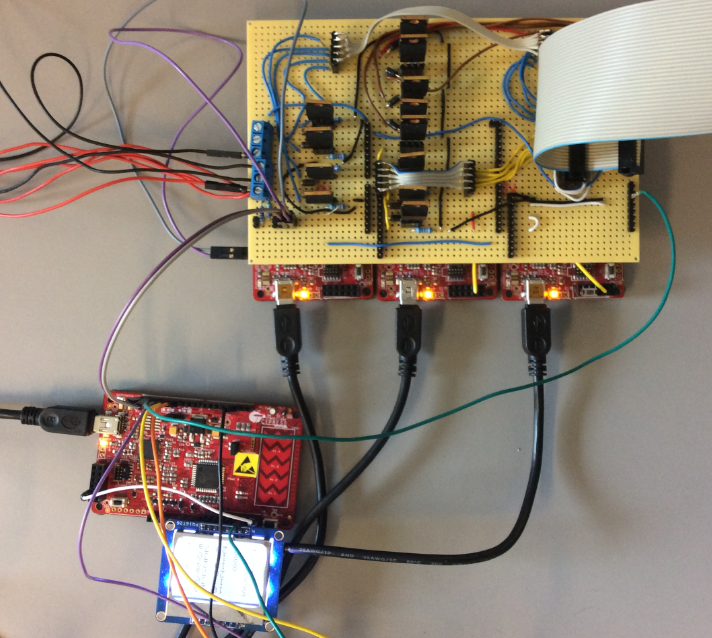
\includegraphics[width=0.4\textwidth]{Filer/FordelingsPrint.PNG}
    \caption{Fordelingsprint}
    \label{fig:Fordelingsprint}
\end{figure}

På figur \ref{fig:Fordelingsprint} ses fordelingsprintet, dette print er bygget med pins så det kan på sættes XY-, Z- og Sensor PSoCs og der med slippe for alt for mange ledninger. Printet indebær, hardwaren til I2C kommunikation mellem PSoC-Master og de resterende PSoCs samt tre motorstyringer til henholdsvis X, Y og Z motorene, der ud over er printet forbundet med motorene, sensorerne og LED'erne via. et 34 lederkabel.

% X Moter Montering
\subsubsection{X Motor Montering}
\begin{figure}[H] \centering
    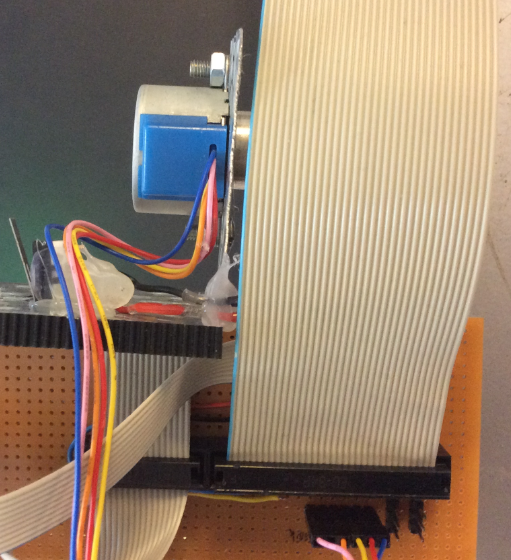
\includegraphics[width=0.3\textwidth]{Filer/XMotorMont.PNG}
    \caption{X Motor Montering}
    \label{fig:XMotorMont}
\end{figure}

På figur \ref{fig:XMotorMont} ses tilslutningen af 34 lederkablet fra fordelerprintet samt monteringen af den ene af X motorene. Fra denne tilslutning bliver signaler, spændinger og kommunikation fordelt ud til deres respektive enheder.

% Z Motor Montering
\subsubsection{Z Motor Montering}
\begin{figure}[H] \centering
    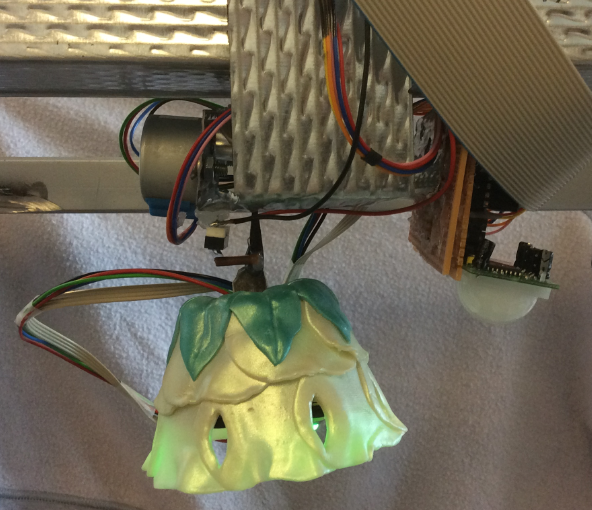
\includegraphics[width=0.3\textwidth]{Filer/ZMotorMont.PNG}
    \caption{Z Motor Montering}
    \label{fig:ZMotorMont}
\end{figure}

På figur \ref{fig:ZMotorMont} ses basen af konstruktionen. Det er her Z motoren, lampen med RGB dioder samt systemets sensorer er monteret.

\subsection{Software}

I projektet er der brugt både C og C++. Alt PSoC software er skrevet i C da det er det sprog PSoC Creator understøtter. Desuden er SPI driveren til DevKit8000 skrevet i C, fordi den er skrevet som et Linux-kernemodul og det kræver igen C. Sidst men ikke mindst er GUI'en på DevKit8000 skrevet i C++ med brug af QT biblioteket.

\subsubsection{Devkit8000}

På Devkit8000 er de mest interessante moduler:

\begin{itemize}
	\item position
	\item light
	\item settings
\end{itemize}

\textbf{Position} er den kodesektion der beskriver, hvordan lampen skal bevæge sig for de tre akser. Kodesektionen håndterer videreførelsen af de beskeder som brugeren opretter gennem position-tabben. Det særligt interessante består i at den grafiske repræsentation, bestående af et koordinatsystem, skal stemme overens med den reele positionering af produktet. Således kan brugeren virtuelt bliver repræsenteret for, hvordan systemet vil blive påvirket såfremt brugeren vælger at realisere disse ved at videresende vha. SPI.

\textbf{Light} er den kodesektion der beskriver lysstyringen for lampens RGB-LED'er. På samme måde som ved position, så viderekommunikeres brugeraktionen på de grafiske elementer til systemet, såfremt dette vælges af brugeren, og genererer desuden en virtuel repræsentation. I dette tilfælde repræsenteres værdierne med en farvepallete med den blandede farve bestående af de tre værdier. Særligt interessant er det her, at repræsentere for brugeren hvordan interaktionen påvirker systemet forinden det bliver viderebragt og påvirker lampens faktiske lys.

\textbf{Settings} kodesektionen står for den generelle sensorkontrol. Man kan her både ved bevægelsessensoren og lumensensoren betragte Devkittet som en afbryder, da disse kun kan ændres til to tilstand, tændt og slukket. Den sidste sensor der påvirkes i denne sektion er afstandssensoren, der altid er aktiv. Denne kan påvirkes med hensyn til, hvilken afstand den skal alarmere resten af systemet. Brugeren får gennem denne sektion frirum til at til eller fravælge sensorfunktionalitet og indstille på dem.

\subsubsection{Master}

Særligt interresant i softwaren på PSoC-Master er \verb+isr_spi_rx()+ og \verb+i2c_tx()+ funktionerne, da de er bærende element i hele funktionaliteten.

\subsubsection{SPI}

%TC:ignore
\lstinputlisting[language=C,caption={isr\_spi\_rx()},label={listing:isrspirx}]{Filer/isr_spi_rx.c}
%TC:endignore

\verb+isr_spi_rx()+ Listing \ref{listing:isrspirx} er en \verb+Interrupt service routine+ som afvikles ved modtagelse af data via SPI-busset. Det modtagede data bliver læst ind på en buffer fra SPI komponenten, derefter deles det op i hhv. en kommando og en værdi. Alt efter hvilken kommando der er modtaget fortages en defineret handling. 


\subsubsection{I2C}

%TC:ignore
\lstinputlisting[language=C,caption={i2c\_tx()},label={listning:i2ctx}]{Filer/i2c_tx.c}
%TC:endignore

\verb+i2c_tx()+ Listing \ref{listning:i2ctx} funktionen bruges til afsendelse af data pakker på I2C-bussen. Når funktionen kaldes sendes der en addresse, kommando og værdi. Kommandoen og værdien sættes ind i en buffer til afsendelse. I bufferen er der også tilføjet en \verb+Start of packet (SOP)+ byte og en \verb+End of packet (EOP)+ byte, disse sættes ind hhv først og sidst i bufferen og bruges af modtageren til at kontrollere om den fulde pakke er modtaget.
Herefter kaldes en \verb+I2CM_I2CMasterWriteBuf()+ med modtager adressen, bufferen til afsendelse, buffer størelsen og mode for afsenelse, som er komplet afsendelse her. Derefter afventer funktionen at pakken er blevet korrekt afsendt og derefter nustiller I2C komponemtets status.


\subsubsection{XY I2C}

%TC:ignore
\lstinputlisting[language=C,caption={I2CS\_I2C\_ISR\_ExitCallback()},label={listning:i2csi2cisrexitcallback}]{Filer/I2CS_I2C_ISR_ExitCallback.c}
%TC:endignore

\verb+I2CS_I2C_ISR_ExitCallback()+ Listing \ref{listning:i2csi2cisrexitcallback} er en \verb+Interrupt service rotine+ som automatisk kaldes efter der er modtaget en data pakke over I2C-busser.
Det modtagede data lagres ind i en struct og alt efter hvilken kommando der er modtaget fortages en defineret handling. Efterfølgende nulstilles SPI komponentens status.

% Sensor
\subsubsection{Sensor}

I PSoC-Sensor er de mest interessante moduler:

\begin{itemize}
	\item handler
	\item LumenSensor
	\item main
\end{itemize}

Modulet \textbf{handler} håndterer PSoC-Sensors opførsel når den modtager I2C kommandoer fra PSoC-Master. Basalt set én stor switch, med en case for hver kommando PSoC-Sensor kan modtage og håndterer.

\textbf{LumenSensor} er det software modul der håndterer I2C kommunikationen med lyssensoren. Dette har fået sit eget modul da en enkelt aflæsning af sensoren består af at skrive en byte til sensoren, læse to bytes fra sensoren, og derefter skrive en og læse to bytes igen.

Sidst men ikke mindst er der \textbf{main}. Den indeholder den overordnede kontrolstruktur i PSoC-Sensor, der bestemmer hvornår alt andet skal køres. Som beskrevet ovenfor i TopDesign, så er hjertet Metronom timeren der giver et taktslag hver halve sekund. For hvert taktslag bliver en række tællere talt op og tjekket for overløb. Hver tæller der løber over bliver nulstillet og hæver et flag. De flag bliver så tjekket i hoved-løkken og den tilhørende kode bliver udført.

Alt i alt giver denne opbygning at der kan defineres periodiske events med individuelle perioder (med en opløsning på 0.5 sekunder). Det giver den fordel at vi kan have en hoved-løkke der kører hele tiden, uden at blive standset af delay kommandoer, hvilket giver muligheden for et mere responsiv og jævnt kørende program. Men samtidig undgår vi at overbelaste sensorene ved at aktiverer dem alt for ofte.

Til sidst bør det nævnes at systemet bruger et \textbf{lux} modul som vi ikke har skrevet selv. Den er kopieret fra lumen sensorens datablad\footcite{TSL2561}.
